\documentclass[10pt,a4paper]{beamer}
\usetheme{Malmoe}
\definecolor{UniGreen}{RGB}{0,150,0}
\setbeamercolor{title}{fg=UniGreen}
\setbeamercolor{frametitle}{fg=UniGreen}
\setbeamercolor{structure}{fg=UniGreen}
\usepackage[utf8]{inputenc}
\usepackage[MeX]{polski}
\usepackage{amsmath}
\usepackage{amsfonts}
\usepackage{amssymb}
\usepackage{graphicx}
\usepackage{rotating}
\usepackage{multirow}
\usepackage{array}
\usepackage{tikz}
\usetikzlibrary{shapes,arrows}
\author{\texorpdfstring{Jakub Turek \newline \href{mailto:jkbturek@gmail.com}{ jkbturek@gmail.com }}{Jakub Turek}}
\title{Wykorzystanie sztucznej inteligencji w grze Scrabble}
\institute{Wydział Elektroniki i Technik Informacyjnych}
\begin{document}

\begin{frame}
	\titlepage
\end{frame}

\section{Wstęp}

\begin{frame}
	\begin{block}{Scrabble}
		\textbf{Gra słowna polegająca na układaniu na określonej planszy wyrazów z~losowanych liter.}
		
		\vspace{10mm}
		
		\emph{Wielki słownik ortograficzny - PWN 2003, 2006, 2008 - E. Polański}
	\end{block}
\end{frame}

\begin{frame}
	\frametitle{Historia Scrabble}
	
	\begin{itemize}
		\item 1938 r. - gra \emph{Lexiko}, Alfred Mosher Butts.
		\item Lata 40. - \emph{Criss-Crossword} - udoskonalona wersja \emph{Lexiko}.
		\item 1948 r. - James Burnot, \emph{Scrabble}.
		\item Lata 80. - Hasbro.
		\item Lata 80. - teleturniej \emph{Scrabble}.
		\item Obecnie - 121 krajów, 29 różnych języków.
		\item Do chwili obecnje - 150 milionów sprzedanych egzemplarzy.
	\end{itemize}
\end{frame}

\subsection{Zasady}

\begin{frame}
	\frametitle{Plansza}
	
	\begin{columns}[onlytextwidth]
		\begin{column}{0.55\textwidth}
			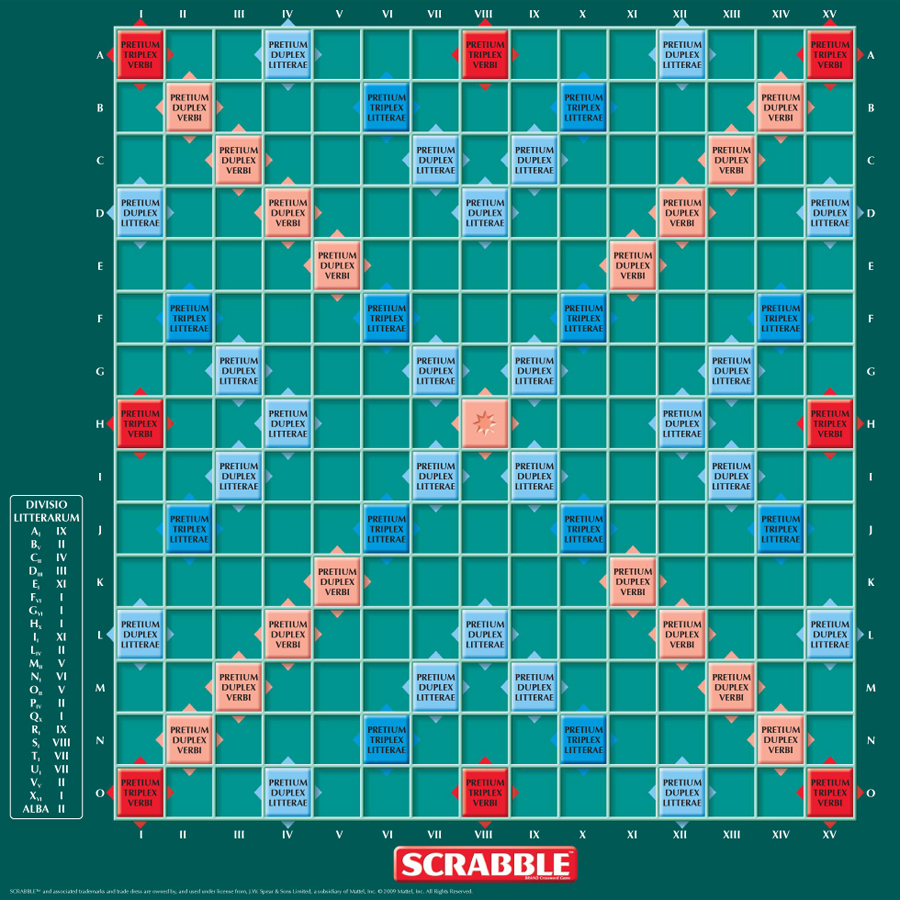
\includegraphics[scale=0.17]{graphics/board.jpg}
		\end{column}
		\begin{column}{0.45\textwidth}
			\begin{itemize}
				\item Wymiary $15 \times 15$.
				\item Premie:
					\begin{itemize}
						\item literowe:
							\begin{itemize}
								\item podwójna,
								\item potrójna.
							\end{itemize}
						\item słowne:
							\begin{itemize}
								\item podwójna,
								\item potrójna.
							\end{itemize}
					\end{itemize}
				\item Środek planszy:
					\begin{itemize}
						\item pierwszy wyraz musi przechodzić przez pole,
						\item podwójna premia słowna.
					\end{itemize}
			\end{itemize}
		\end{column}
	\end{columns}
\end{frame}

\begin{frame}
	\frametitle{Płytki (polska wersja)}
	
	\begin{columns}[onlytextwidth]
		\begin{column}{0.55\textwidth}
			\scalebox{0.8}{
				\begin{tabular}{|c|c|c||c|c|c||c|c|c|}
					\hline
					\multirow{16}{*}{
						\begin{sideways}
							Litera
						\end{sideways}	} &
					\multirow{16}{*}{
						\begin{sideways}
							Ilość płytek
						\end{sideways}} & 
					\multirow{16}{*}{
						\begin{sideways}
							Liczba punktów
						\end{sideways}} & \textbf{A} & 9 & 1 & \textbf{M} & 3 & 2 \\
					\cline{4-9}
					&&& \textbf{Ą} & 1 & 5 & \textbf{N} & 5 & 1 \\
					\cline{4-9}
					&&& \textbf{B} & 2 & 3 & \textbf{Ń} & 1 & 7 \\			
					\cline{4-9}
					&&& \textbf{C} & 3 & 2 & \textbf{O} & 6 & 1 \\			
					\cline{4-9}
					&&& \textbf{Ć} & 1 & 6 & \textbf{Ó} & 1 & 5 \\
					\cline{4-9}
					&&& \textbf{D} & 3 & 2 & \textbf{P} & 3 & 2 \\	
					\cline{4-9}
					&&& \textbf{E} & 7 & 1 & \textbf{R} & 4 & 1 \\
					\cline{4-9}
					&&& \textbf{Ę} & 1 & 5 & \textbf{S} & 4 & 1 \\
					\cline{4-9}
					&&& \textbf{F} & 1 & 5 & \textbf{Ś} & 1 & 5 \\
					\cline{4-9}				
					&&& \textbf{G} & 2 & 3 & \textbf{T} & 3 & 2 \\
					\cline{4-9}
					&&& \textbf{H} & 2 & 3 & \textbf{U} & 2 & 3 \\
					\cline{4-9}
					&&& \textbf{I} & 8 & 1 & \textbf{W} & 4 & 1 \\
					\cline{4-9}
					&&& \textbf{J} & 2 & 3 & \textbf{Y} & 4 & 2 \\
					\cline{4-9}
					&&& \textbf{K} & 3 & 2 & \textbf{Z} & 5 & 1 \\
					\cline{4-9}
					&&& \textbf{L} & 3 & 2 & \textbf{Ź} & 1 & 9 \\
					\cline{4-9}
					&&& \textbf{Ł} & 2 & 3 & \textbf{Ż} & 1 & 5 \\
					\hline
				\end{tabular}
			}
		\end{column}
		\begin{column}{0.45\textwidth}
			\begin{itemize}
				\item 98 płytek z~literami.
				\item Każda litera ma przyporządkowaną punktację.
				\item Ilość płytek proporcjonalna do częstotliwości występowania litery.
				\item Punktacja odwrotnie proporcjonalna do częstotliwości występowania litery.
				\item 2 \emph{blanki}.
			\end{itemize}
		\end{column}
	\end{columns}
\end{frame}

\begin{frame}
	\frametitle{Reguły}
	
	\begin{itemize}
		\item Na stojaku 7 wylosowanych płytek.
		\item Naprzemienne ruchy.
		\item Prawidłowy ruch:
			\begin{itemize}
				\item Płytki wyłożone w~jednym wierszu (lub kolumnie) w~sposób ciągły.
				\item Wykorzystanie przynajmniej jednej litery znajdującej się już na planszy.
				\item Tworzy poprawny wyraz czytany od lewej do prawej (lub od góry do dołu).
				\item Wszystkie płytki przylegające tworzą poprawne wyrazy w~układzie krzyżówkowym.
			\end{itemize}
		\item Koniec gry - pierwszy gracz, który nie ma płytek na stojaku.
		\item Wygrywa gracz z~największą liczbą punktów.
	\end{itemize}
\end{frame}

\begin{frame}
	\frametitle{Dopuszczalne słowa}
	
	Dopuszczalne jest wykorzystanie wszystkich słów znajdujących się w~dowolnym słowniku języka polskiego (wraz z~poprawnymi odmianami) z~wyłączeniem:
	
	\begin{itemize}
		\item nazw własnych (wyrazów pisanych z~wielkiej litery),
		\item skrótów,
		\item przedrostków, przyrostków,
		\item wyrazów wymagających użycia apostrofu lub łącznika.
	\end{itemize}
\end{frame}

\section{Słowniki}
\subsection{Polskie słowniki wyrazów do gier}

\begin{frame}[fragile]
	\frametitle{Słownik wyrazów do gier}
	
	\textbf{Słownik wyrazów do gier} to lista wszystkich słów, wraz ze wszystkimi poprawnymi odmianami, dopuszczalnych do wykorzystania w~grach słownych. 
	
	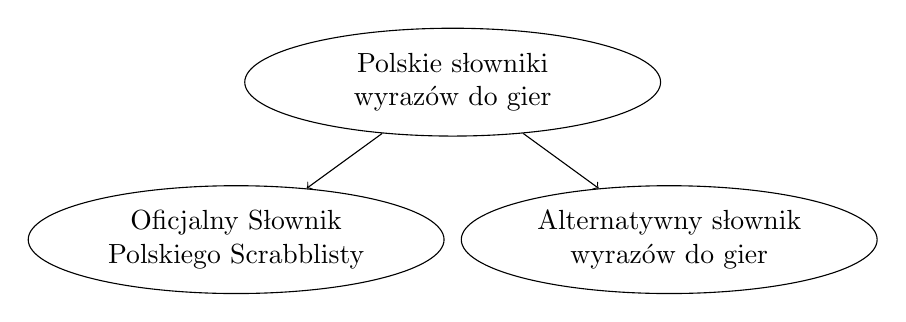
\begin{tikzpicture}
		\tikzstyle{every node}=[draw, shape=ellipse, text width=3.5cm, align=center];
		\node (alternative) at (2.75, -2) {Alternatywny słownik wyrazów do gier};
        \node (pfs) at (-2.75, -2) {Oficjalny Słownik Polskiego Scrabblisty};
		\node (dictionaries) at (0, 0) {Polskie słowniki wyrazów do gier};
		\draw[->] (dictionaries) -- (pfs);
		\draw[->] (dictionaries) -- (alternative);
	\end{tikzpicture}
\end{frame}

\begin{frame}
	\frametitle{Porównanie OSPS i~słownika alternatywnego}
	
	\scalebox{0.75}{
		\begin{tabular}{|l|c|c|}
			\cline{2-3}
			\multicolumn{1}{c|}{} & \textbf{OSPS} & \textbf{Słownik alternatywny} \\
			\hline
			\multirow{2}{*}{Wydawca} & Polska Federacja Scrabble, & \multirow{2}{*}{Serwis z~grami online Kurnik} \\
			& Polskie Wydawnictwo Naukowe & \\
			\hline
			Przeznaczenie & Gry turniejowe & Gra ,,Literaki'' \\
			\hline
			Liczba słów & 2 477 212 & 2 703 830 \\
			\hline
			\multirow{3}{*}{Źródło} & Zamknięta lista słowników języka & Otwarta lista słowników języka \\
			& polskiego, ortograficznych, wyrazów & polskiego, ortograficznych, \\
			& obcych wydawnictwa PWN & wyrazów obcych \\
			\hline
			\multirow{6}{*}{Przykładowe różnice} & \multicolumn{1}{l|}{\textcolor{UniGreen}{$\blacktriangleright$} basfu}  & \multicolumn{1}{l|}{\textcolor{UniGreen}{$\blacktriangleright$} aeolipile} \\
			& \multicolumn{1}{l|}{\textcolor{UniGreen}{$\blacktriangleright$} gral} & \multicolumn{1}{l|}{\textcolor{UniGreen}{$\blacktriangleright$} donowi} \\
			& \multicolumn{1}{l|}{\textcolor{UniGreen}{$\blacktriangleright$} meru} & \multicolumn{1}{l|}{\textcolor{UniGreen}{$\blacktriangleright$} feroce} \\
			& \multicolumn{1}{l|}{\textcolor{UniGreen}{$\blacktriangleright$} noblów} & \multicolumn{1}{l|}{\textcolor{UniGreen}{$\blacktriangleright$} geez} \\
			& \multicolumn{1}{l|}{\textcolor{UniGreen}{$\blacktriangleright$} późńmyż} & \multicolumn{1}{l|}{\textcolor{UniGreen}{$\blacktriangleright$} tyiyn} \\
			& \multicolumn{1}{l|}{\textcolor{UniGreen}{$\blacktriangleright$} szwed} & \multicolumn{1}{l|}{\textcolor{UniGreen}{$\blacktriangleright$} żad} \\
			\hline
		\end{tabular}
	}
	
\end{frame}

\end{document}